
前一章中,我们研究了CPU资源,以及如何使用它们以获得最佳性能。我们观察到CPU有能力并行执行大量指令(指令级并行)。在多个基准测试中看到了CPU可以在每个周期中执行许多操作,而不会造成任何性能损失,例如:添加和减去两个数字所花费的时间与添加两个数字所消耗的时间一样。

但读者们可能已经注意到,这些基准测试和示例具有一个相当不同寻常的特性。参考以下例子:

\begin{lstlisting}[style=styleCXX]
for (size_t i = 0; i < N; ++i) {
	a1 += p1[i] + p2[i];
	a2 += p1[i] * p2[i];
	a3 += p1[i] << 2;
	a4 += p2[i] – p1[i];
	a5 += (p2[i] << 1)*p2[i];
	a6 += (p2[i] - 3)*p1[i];
}
\end{lstlisting}

我们已经用这段代码演示了CPU可以对这两个值\texttt{p1[i]}和\texttt{p2[i]}进行8次操作,与只进行一次操作的开销几乎相同。但我们要非常小心地添加更多的操作,而非添加更多的输入;某些情况下,只要这些值已经在寄存器中,CPU的内部并行性就会启用。前面的示例中,在添加第二个、第三个……直到第8个操作时,我们只保留两个输入。这将导致一些不常见的代码。现实中,对于给定的一组输入,需要计算的有多少?大多数时候都不到8个。

这并不意味着CPU的计算潜力被浪费了,除非碰巧运行了前面示例中的奇异代码。指令级并行性是流水线的计算基础,流水线可以同时执行循环中不同迭代的操作。无分支计算是用条件指令换取无条件计算,因此我们可以获得更多的“不耗时”计算。

然而,问题仍然存在:为什么要以这种方式限制CPU的基准测试?毕竟,之前的例子中,如果添加更多输入,便能够更轻松地想出8种不同的内容:

\begin{lstlisting}[style=styleCXX]
for (size_t i = 0; i < N; ++i) {
	a1 += p1[i] + p2[i];
	a2 += p3[i] * p4[i];
	a3 += p1[i] << 2;
	a4 += p2[i] - p3[i];
	a5 += (p4[i] << 1)*p2[i];
	a6 += (p3[i] - 3)*p1[i];
}
\end{lstlisting}

这与前面看到的代码相同,只是现在每次迭代操作4个不同的输入值,而不是两个。其继承了前面例子中所有的笨拙,但仅是因为我们希望在测量某些变化对性能的影响时尽可能少地进行更改。其对性能的影响还挺大:

%\hspace*{\fill} \\ %插入空行
\begin{center}
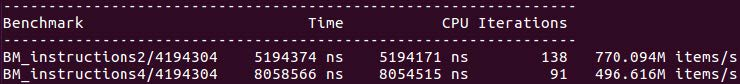
\includegraphics[width=0.9\textwidth]{content/1/chapter4/images/1.jpg}\\
图 4.1
\end{center}

对4个输入值进行相同的计算,大约要多花36\%的时间。当需要访问内存中的数据时,计算就会延迟。

应该注意的是,添加更多的自变量、输入或输出可能会影响性能的原因是:CPU可能正在消耗用于存储这些变量进行计算的寄存器。虽然这在许多实际的程序中是一个问题,但在这里不是。这里的代码不够复杂,不足以占满现代CPU的所有寄存器(确认这一点的最简单方法是检查机器码)。

显然,访问更多的数据似乎会降低代码的速度。为什么呢?高层次的原因是内存跟不上CPU的计算速度。有几种方法可以估计这种速率的差异。最简单的方法在现代CPU的参数表中进行查阅。现在的CPU的时钟频率在3GHz到4GHz之间,一个周期大约是0.3纳秒。在适当的情况下,CPU可以每秒执行几个操作,所以每纳秒执行10个操作并是可能的(尽管在实践中很难实现,这是一个非常有效的程序的可靠标志)。另一方面,内存则慢得多,例如:DDR4内存的工作频率为400Mhz。你也可以找到高达3200MHz的值。无论如何,这不是内存时钟,而是数据速率,要将其转换为类似于内存传输数据的速度,还必须考虑\textbf{列访问频闪延迟},通常称为\textbf{CAS延迟}或\textbf{CL}。简单来说,这是RAM接收数据请求、处理数据并返回值所需的周期数。没有在所有情况下都有意义的内存速度定义(本章后面,我们将看到一些原因),但是,对于数据速率为3.2GHz和CAS延迟15的DDR4模块来说,其内存速度大约是107MHz,即每次访问9.4需要纳秒。

无论从哪个角度来看,CPU每秒执行的操作要比内存为这些操作提供输入值或存储结果的能力多。程序需要以某种方式使用内存,访问内存的细节将对性能产生重大影响,有时甚至会限制内存。然而,内存速率差对性能的影响会从微不足道到成为程序的瓶颈。所以,必须了解不同条件下的内存如何影响程序性能,以及原因是什么,这样就可以利用这些知识来设计和优化我们自己的代码,从而获得最佳性能。








